\section{Zielsetzung}
\label{sec:Zielsetzung}
In diesem Versuch wird die Beugung einer Lichtwelle am Einzel- und Doppelspalt analysiert und die entsprechenden Beugungsfiguren gemessen und dargestellt.

\section{Theorie}
\label{sec:Theorie}
Nimmt Licht Wellencharakter an, kann mit den Huygensschen Prinzip das Auftreten von Beugungseffekten an einem Spalt erklärt werden.
Das Prinzip besagt, dass an jeder Stelle einer Wellenfläche neue Elementarwellen entstehen, welche Kugelwellen sind. Sie interferieren miteinander und erzeugen eine neue Wellenfront. 
Bei der Beugung breitet sich das Licht in andere Richtungen unter einem Winkel aus. Es gibt zwei Arten von Beugung, in diesem Versuch wird nur die Fraunhofer Beugung betrachtet, da mit ihr mathematisch leichter gerechnet werden kann. 
Dort werden die Strahlen unter dem gleichen Winkel abgelenkt und das Licht tritt parallel auf den Spalt, anders als bei der Fresnel Beugung(s. Abbildung 1).
Die Länge des Spalts ist groß gegen seine Breite b und die Quelle befindet sich theoretisch im Unendlichen.
\begin{figure}[H]
  \centering
  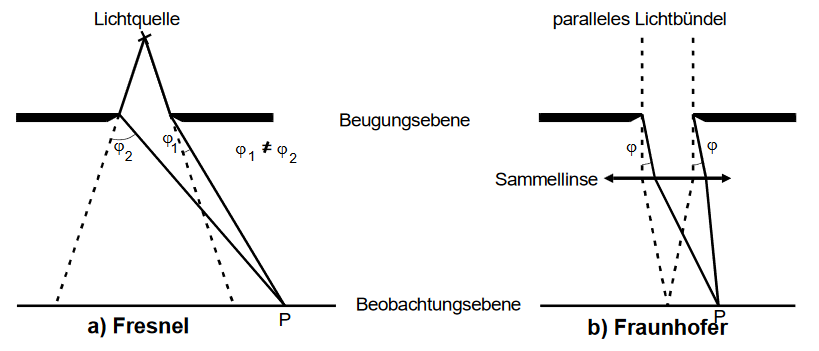
\includegraphics[height=5cm]{naherung.PNG}
  \caption{Fraunhofer- und Fresnel Beugung im Vergleich.\cite{kent}.}
\end{figure}
\noindent Aus der Überlagerung der Elementarwellen, lässt sich der Schwingungszustand eines Punktes im Wellenfeld einer einfallenden ebenen Welle der Form $A(z, t) = A_0 \symup{exp}(\symup{i}(\omega t -2\pi z/\lambda))$ 
bestimmen. Hierbei ist $\lambda$  die Wellenlänge und $z$ die Richtung.
Die Phasendifferenz zweier Strahlenbündel, die von zwei Punkten mit dem Abstand $x$ ausgehen, berechnet sich durch
\begin{align}
  \delta = \frac{2\pi s}{\lambda} = \frac{2\pi x \sin{\varphi}}{\lambda}
\end{align}
wobei $s$ den Wegunterschied beschreibt.
Die Amplitude $B$ in $\varphi-$Richtung berechnet sich durch
\begin{align}
  B(z,t, \varphi) = A_0 \symup{e}^{\symup{i} \left(\omega t - \frac{2\pi z}{\lambda} \right)} e^{\frac{\pi \symup{i} b \sin{\varphi}}{\lambda}} \frac{\lambda}{\pi \sin{\varphi}}
  \sin{\left(\frac{\pi b \sin{\varphi}}{\lambda}\right)}
\end{align}
Allerdings sind nur die letzten beiden Faktoren relevant für diesen Versuch. Somit lässt sich die Amplitude in Abhängigkeit von $\varphi$ mit der Abkürzung $\eta = \frac{\pi b sin \varphi}{\lambda}$ schreiben als
\begin{align}
   B(\varphi) = A_0 b \frac{sin \eta}{\eta}.
\end{align}
Die Gestalt dieser Beugungsfigur für deinen Parallelspalt ist in Abbildung 2 dargestellt.
Die Funktion hat also lokale Maxima und Minima, die sich immer näher an Null annähern.
Es kann nur die zeitlich gemittelte Intensität gemessen werden, da die Lichtfrequenz zu hoch ist. Die Intensität ist proportional zum Quadrat der Amplitude
\begin{align}
  I(\varphi) \propto B(\varphi)^2 = A_0^2 b^2 \left(\frac{\lambda}{\pi b \sin{\varphi}} \right)^2  \sin^2{\left(\frac{\pi b \sin{\varphi}}{\lambda}\right)}
\end{align}
\begin{figure}[H]
  \centering
  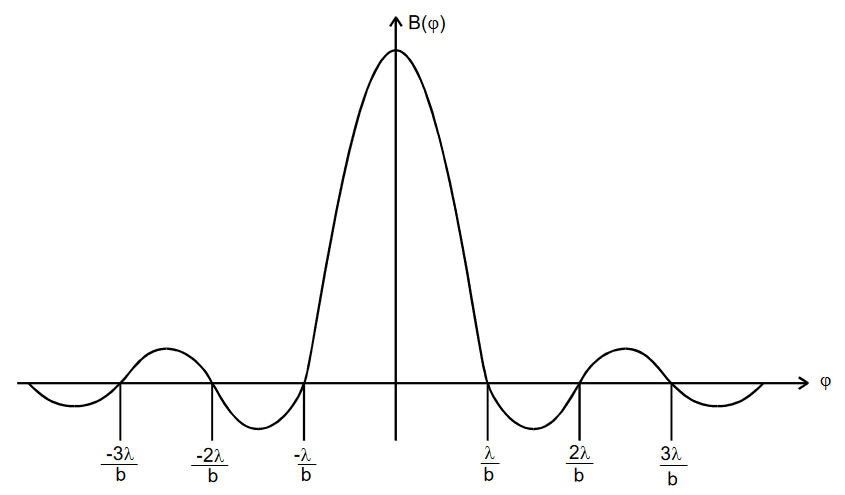
\includegraphics[height=6cm]{beugung.PNG}
  \caption{Amplitude einer an einem Spalt gebeugten Welle in Abhängigkeit von dem Winkel $\varphi$.\cite{kent}.}
\end{figure}

\noindent Die Intensität für einen Doppelspalt kann als Überlagerung zweier Einfach-Spalte mit Breite $b$ und Abstand $s$ gesehen werden
\begin{align}
   I(\varphi) \propto B(\varphi)^2 = 4 \cos^2{\left(\frac{\pi s \sin{\varphi}}{\lambda}\right)} \left(\frac{\lambda}{\pi b \sin{\varphi}}\right)^2
   \sin^2{\left(\frac{\pi b \sin{\varphi}}{\lambda}\right)}
\end{align}
Zusätzliche Nulldurchgänge werden also auch auf Grund der $cos^2$-Verteilung gemessen.
